\documentclass[12pt]{article}
\usepackage{graphicx}
\usepackage[hidelinks]{hyperref}

\graphicspath{ {./images/} }

\begin{document}

\title{Formulario Segnali}
\author{Giuliano Vallone}
\date{}
\maketitle

\tableofcontents
\newpage

\section{Software requirement Specifications}
\subsection{Introduction}
\subsubsection{Aim of the document}
The main focus of this document is to describe the steps of the design of this system, named CTFun. 
\subsubsection{Overview of the defined system}
The system here described is an application that provides a training platform for players of Capture The Flag, with some features for competition, like a scoreboard accessible from all players that can encourage competitiveness between players. 
\subsubsection{Hardware and Software requirements}
The hardware requirements for this platform to work properly are an Internet connection and enough resources for manage multiple HTTP connections. Also will require a good amount of free disks for upload the challenges on the machine that will host this software. It is not required to use an external server for hosting a DBMS.
For software requirements it will be required to have a working JRE (21 at least) correctly installed on the host. For the DB, the application will initialize it with SQLite by default so it won't be necessary to install DBMS server.
\subsubsection{Related Systems, Pros and Cons}
The other systems related to CTFun are:
\begin{itemize}
\item Google
\item Facebook
\end{itemize}
Since this two system have the same function with CTFun, their pros and cons of this two will be described together. The pros are that a user (player or admin) won't have to create an account for login in the platform, so basically for him is just a password less to memorize. The cons are Google and Facebook are not trustworthy in matter of privacy and this will add more code to write for implement their API.
\subsection{User Stories}
\begin{itemize}
\item As a player, I want to read the description of a challenge, so i can search for external material to study on for solve the challenge
\item As a player, I want to see a global scoreboard, so i can measure myself with other players on the platform
\item As an admin, I want to be able to change the flag of a challenge
\end{itemize}
\subsection{Function Requirements}
\begin{itemize}
\item The system shall provide a scoreboard accessible by all players
\item The system shall provide a login for non registered players
\item The system shall provide a description and a link for every attachment of the challenge when a player selects it
\end{itemize}
\subsection{Use Cases}
\subsubsection{Overview Diagram}
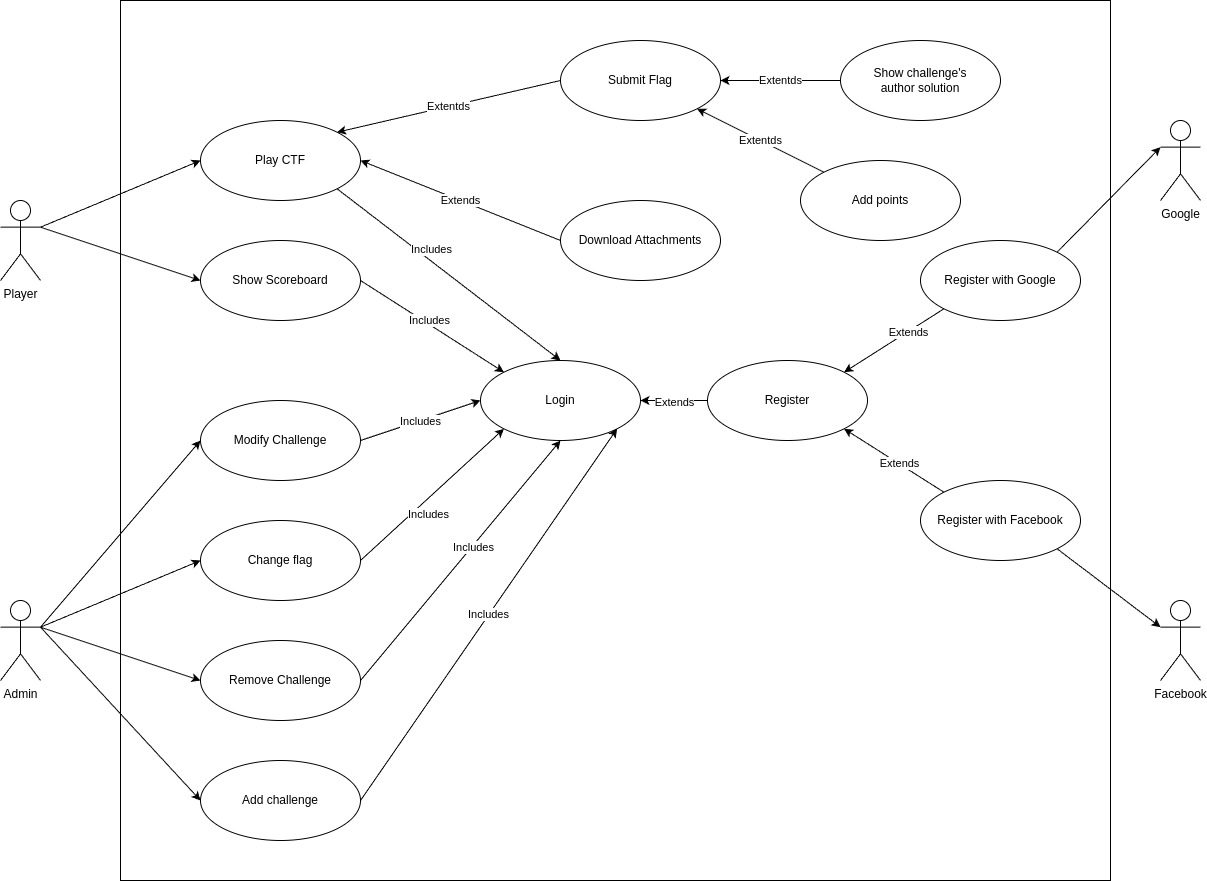
\includegraphics[scale=0.4]{Use Case Diagram.jpg}
\subsubsection{Internal Steps}
\paragraph{Name: Play CTF}
\begin{itemize}
\item[1.] The player selects a challenge.
\item[2.] The system shows a description of the challenge and a blank box for the flag.
\item[3.] The player submits the flag.
\item[4.] The system checks the correctness of the flag.
\item[5.] The system adds the points to player's score.
\item[6.] The system shows a link for the solution of the challenge's author.
\item[7.] The player clicks the link.
\item[8.] The system shows the official write up.
\end{itemize}
\paragraph{Extensions}
\begin{itemize}
\item [1a.] \textit{The challenge is not available at the moment}: The system notifies the player and terminates the use case.
\item [2a.] \textit{The challenge has one or more attacchemnts}: The system shows a link for download the attachments.
\item [4a.] \textit{The flag is not correct}: The system notifies the player that the flag is not correct.
\end{itemize}
\section{Storyboards}
\section{Design}
\subsection{Class Diagram}
\subsubsection{VOPC}
\subsubsection{Design-Level Diagram}
\subsection{Design Patterns}
\subsection{Activity Diagram}
\subsection{Sequence Diagram}
\subsection{State Diagram}
\section{Testing}
\section{Exceptions}
\section{Persistance}
\section{Sonar Cloud}
\end{document}